\documentclass{hfscript}
\usepackage{hyperref}       % Für klickbare Links in PDF
\usepackage{booktabs}       % Für schönere Tabellen mit top-/mid-/bottomrule
\usepackage{tabularx}       % Für Tabellen mit fixer Breite
\usepackage{multirow}       % Für Tabellenzellen über mehrere Spalten/Zeilen
\usepackage{textcomp}       % Für Symbole, zb. Copyright
\usepackage{lastpage}       % Für \lastpage
\usepackage{graphicx}       % Für Bilder
\usepackage{amsmath}        % Für Mathematik
\usepackage{amssymb}        % Für Mathesymbole
\usepackage{pifont}         % Einige Mathe-Befehle benötigen dieses Paket für Symbole
\usepackage{cancel}         % Zum Durchstreichen mit \cancel,\bcancel,\xcancel
\usepackage{placeins}       % Für \FloatBarrier
\usepackage{wrapfig}        % Für Bilder mit Text drumrum
\usepackage{pdfpages}       % PDF Seiten einfügen

%% Glossary
\usepackage[toc,xindy,numberedsection]{glossaries}
\loadglsentries[main]{glossar}
\makeglossaries
\glossarystyle{listgroup}
%% Wenn ein Quellenverzeichnis genutzt wird, die folgende Zeile unkommentieren
\usepackage{csquotes}               % Biblatex verlangt dieses Paket.
\usepackage[style=apa]{biblatex}    % Für Quellenverzeichnis
\DeclareLanguageMapping{ngerman}{ngerman-apa}
\addbibresource{quellen.bib}

%% Zwingende Variablen, damit Vorlage korrekt funktioniert
\title{Zusammenfassung}
\subtitle{Flashspeicher}
\hfsem{Frühjahrssemester 2018}
\hffach{Computer Hardware}
\dozent{André Mangold}
\author{Nicolas Haenni}
\date{\today}

\begin{document}
%% Titelseite / Erste Seite
%% Page Style anders, damit Kopf-/Fußzeilen passen
\thispagestyle{scrheadings}
%%%%%%%%%%%%%%%%%%%%%%%%%%%%%%%%%%%%%%%%%%%%%%%%%%%%%%%%%%
%% Titel-Stil

%% Short Title
%% Titel ist nur oben auf der ersten Seite, Inhalt kann
%% direkt auf der ersten Seite starten.

%\maketitle

%% Long Title
%% Es gibt eine Titelseite. Inclusive Abstrakt 
%% (Zusammenfassung), Dokumenten-Management und
%% Lizenzangabe.

\maketitle
\begin{abstract}
    Zusammenfassung zum Thema \emph{Flashspeicher}. Ein Vortrag von Nicolas Haenni, Stoff für die zweite Prüfung des zweiten Semesters im Fach Computer Hardware an der HF-ICT.
\end{abstract}

\subsection*{Dokumentenhistorie}
\begin{center}
    \begin{tabularx}{.9\textwidth}{llX}
        \toprule
        \textbf{Version} & \textbf{Datum} & \textbf{Beschreibung} \\
        \midrule
        0.1 & 05.04.2018 & Erstellen des Dokumentes \\
            &			 & Kapitel Funktionsprinzip erstellt \\
        0.2 & 06.04.2018 & Technischer Aufbau geschrieben \\
        \bottomrule
    \end{tabularx}
\end{center}

\vfill

\footnotesize{Dieses Dokument steht unter der GNU General Public Free Document License (GPL FDL). Weitere Informationen unter https://www.gnu.org/licenses/fdl.html.}
\clearpage
%%%%%%%%%%%%%%%%%%%%%%%%%%%%%%%%%%%%%%%%%%%%%%%%%%%%%%%%%%
%% Inhaltsverzeichnis
%% Wenn ein Inhaltsverzeichnis benötigt wird, die folgende
%% Zeile unkommentieren
%% Für Seitenumbruch nach dem Inhaltsverzeichnis beide
%% Zeilen unkommentieren.
\tableofcontents
\clearpage

% Separate Kapitel können per input eingebunden werden.
\section{Vorwort}
\section{Geschichte}
\section{Technischer Aufbau}
Flash-Speicher basiert auf sogenannten Floating Gate-Transistoren (FGFET). Die Basis für diese sind die sogenannten Metal-Oxid-Halbleiter-Feldeffekttransistoren, kurz MOSFET. In diesem Kapitel wird der physikalische Aufbau zuerst des MOSFETs und anschließend des Floating Gate-Transistors eingegangen. Die Funktionsweise wird im folgenden Kapitel \ref{sec:funktion} beschrieben.

\subsection{Metal-Oxid-Halbleiter-Feldeffekttransistor}
\begin{figure}[h]
    \centering
    \caption{MOSFET als Bauteil}
    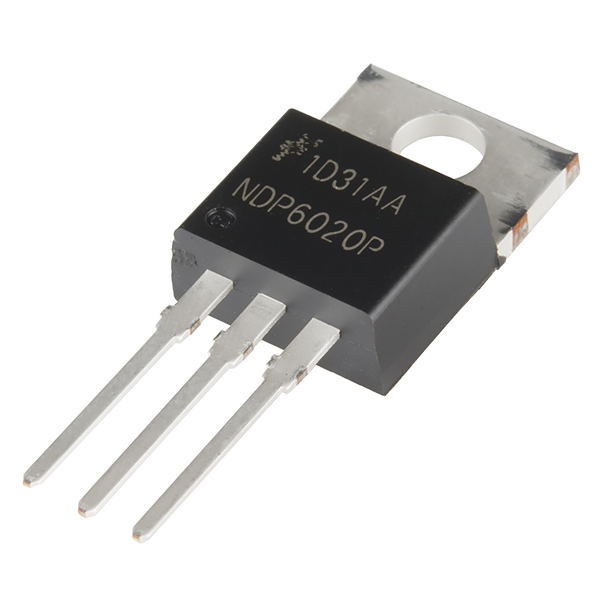
\includegraphics[width=5cm]{sections/img/mosfet_bauteil}
    \label{fig:mosfet.bauteil}
    \\ Quelle: \cite{mosfetshop}
\end{figure}

Ein MOSFET besteht aus einer Art Grundplatte, welche aus einer \gls{pdotiert}en Siliziumeinkristal als Substrat besteht. In dieses Substrat befinden sich zwei stark \gls{ndotiert}e Inseln in denen sich die \emph{Source}-\footnote{dt.: Quelle} und \emph{Drain}\footnote{dt.: Abfluss}-Elektroden befinden. Der Bereich zwischen den beiden Elektroden ist das \gls{pdotiert}e Substrat. Dadurch ist ein Stromfluss zwischen den beiden Elektroden grundsätzlich nicht möglich.

\begin{figure}[h]
    \centering
    \caption{Aufbau eines MOSFETs}
    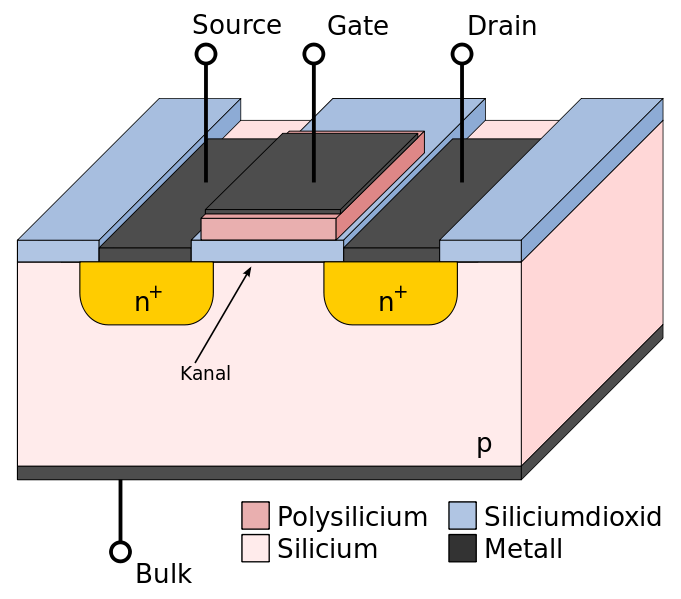
\includegraphics[width=5cm]{sections/img/mosfet_aufbau}
    \label{fig:mosfet.aufbau}
    \\ Quelle: \cite{mosfetwiki}
\end{figure}

Über der Fläche befindet sich eine dünne, isolierende Schicht -- meistens aus Siliziumdioxid. auf dieser Isolierschicht befindet sich dann ein Gate-Material aus \gls{dotiert}em Polysilizium.

\subsection{Floating Gate-Feldeffekttransistor}\label{sec:fgfet}
Die Speicherzellen in Flash-Speicher bestehen aus Floating Gate-Feldeffekttransistoren, kurz FGFET. Diese sind eine Art Weiterentwicklung der MOSFET.

Der Aufbau des FGFETs ist dem des MOSFET sehr ähnlich, allerdings befindet sich zwischen dem Substrat und der Gate-Elektrode noch eine weitere Schicht, das so genannte \emph{Floating Gate}.

\begin{figure}[h]
    \centering
    \caption{Aufbau eines Floating Gate-Transistors}
    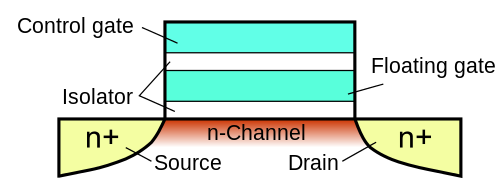
\includegraphics[width=5cm]{sections/img/fgfet_aufbau}
    \label{fig:fgfet.aufbau}
    \\ Quelle: \cite{fgfetwiki}
\end{figure}

Der Name \emph{Floating Gate} stammt daher, dass es rundherum komplett eletrkisch isoliert ist. Es schwebt elektrisch gesehen zwischen der oberen Isolationsschicht des Substrates und der Gate-Elektrode.
\section{Funktionsprinzip}\label{sec:funktion}

Um Daten auf einem Flash-Speicher nicht-flüchtig sichern zu können, werden die Ladezustände der einzelnen Bits auf so genannten \emph{Floating Gates} auf einer Art speziellen Transistor abgelegt. 

Die Ladung dieser Floating Gates sorgt schlussendlich dafür, dass die unterhalb dessen angebrachten Kontakte für \emph{Source} und \emph{Drain} leitend verbunden sind oder nicht.

\subsection{MOS-Feldeffekttransistor}

Die Grundlage für den Floating-Gate-Transistoren (FGMOS) ist der MOSFET. Dieser existiert in verschiedenen Varianten: Anreicherungs- und Verarmungstyp, sowie \gls{ndotiert} und \gls{pdotiert}.

Wie aus Kapitel \ref{sec:fgfet} ersichtlich befindet sich der MOSFET grundsätzlich in einem Sperrzustand. Dies bedeutet, dass die Verbindung zwischen Source- und Drain-Anschluss nicht leitend ist. Um diesen leitend zu machen, wird eine Spannung zwischen Source- und Gate-Anschluss angelegt.

Dadurch werden aus dem umgebenden p-dotierten Substrat (viele Löcher, wenig Elektronen) die verbliebenen Elektronen in den Bereich unter dem Gate-Anschluss gezogen. So entsteht unter dem Gate und zwischen Source und Drain ein leitender Kanal, dessen Leitfähigkeit durch die Spannung am Gate gesteuert werden kann (s. Abbildung \ref{fig:mosfetleitend}).

\begin{figure}[h]
    \centering
    \caption{Leitender Gang im MOSFET bei Spannung am Gate}
    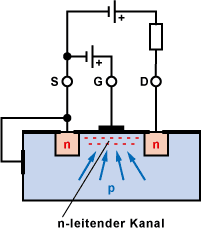
\includegraphics[width=5cm]{sections/img/mosfet2}
    \label{fig:mosfetleitend}
    \\ Quelle: \cite{mosfetkomp}
\end{figure}

Die Spannung, die am Gate benötigt wird, um die Verbindung zwischen Source und Drain herzustellen, nennt sich \emph{Schwellspannung}.

Der Verarmungstyp ist immer leitend, da eine leicht n-dotierte Schicht zwischen den ebenfalls n-dotierten Source- und Drain-Inseln angebracht ist. Er wird sperrend (nicht-leitend) wenn die Gatespannung negativer ist als die Spannung am Source-Anschluss.

Zusammenfassend lässt sich sagen, dass ein MOSFET wie ein Schalter ist: Liegt eine Spannung am Gate an, dann wird die Verbindung zwischen Source und Drain leitend. Liegt keine Spannung am Gate an, dann ist die Verbindung zwischen Source und Drain getrennt.

\subsection{Floating Gate-Transistor}

Der Floating Gate-Transistor ist eine Art leicht abgewandelter MOSFET.  Das Floating Gate, welches sich elektrisch isoliert zwischen dem Substrat und der Gate-Elektrode befindet, kann eine Ladung speichern und diese mehrere Jahre erhalten.

Um das Floating Gate zu laden, macht man sich den quantenmechanischen Tunneleffekt zur Nutze. Dieser ermöglicht es, eine Ladung durch eine nicht-leitende Schicht hindurch zu transportieren (in Anlehnung an \parencite{tunneleffektwiki}).

Um das Floating Gate zu laden, wird eine viel stärkere Spannung an Source und Gate angelegt, als die Schwellspannung, die "`zum Öffnen des Schalters"' nötig wäre (z.B.: 10V anstatt 3,3V). Dadurch wandern Elektronen durch die isolierende Schicht des Floating Gates in dieses. Da es jedoch isoliert ist, können diese nicht mehr "`abfließen"' -- das Floating Gate bleibt geladen.

Ist nun das Floating Gate geladen, wirkt es gleich wie ein MOSFET, bei dem Spannung an das Steuerungsgate gelegt wird: Die Verbindung zwischen Source und Drain wird leitend (angelehnt an \parencite{quora}).

Um den Wert im FGFET auszulesen muss nun nur überprüft werden, ob die Verbindung zwischen Source und Drain leitend ist oder nicht.

\subsection{NAND- und NOR-Speicher}



\subsection{SLC-, MLC- und TLC-Flash-Speicher}
Das Floating Gate der Single-Level-Cell ist nur in der Lage zwei Zustände -- geladen und ungeladen -- anzunehmen. Aus Platzgründen begann man damit, mehrere Zustände in einem Floating Gate zu speichern.

So entstanden die Multi-Level-Zellen. Diese sind in der Lage, zwei Bits zu speichern, können also vier Zustände annehmen, wobei jeder Zustand einer unterschiedlich großen Ladung entspricht.

Analog dazu können Triple-Level-Zellen drei Bit speichern. Eine Übersicht über die verschiedenen Zellen gibt die folgende Tabelle \ref{tab:slcmlc}.

\begin{table}[h]
    \centering
    \caption{Übersicht über SLC-, MLC und TLC-Flash-Speicher}
    \begin{tabular}{p{3cm}|l|l|l}
        & \textbf{Single Level Cell} & \textbf{Multi Level Cell} & \textbf{Triple Level Cell} \\ \hline
        \textbf{Bit pro Zelle} & 1 Bit & 2 Bit & 3 Bit \\ \hline
        \textbf{Speicherbare Zustände} & 2 ($2^1$) & 4 ($2^2$) & 8 ($2^3$) \\ \hline
        \textbf{Lebensdauer} & 100'000 Schreibvorgänge & 3'000 Schreibvorgänge & ca. 1'000 Schreibvorgänge \\ \hline
        \textbf{Fehlerrate} & sehr niedrig & mittel & hoch \\ \hline
        \textbf{Geschwindigkeit} & sehr hoch & niedrig & niedrig \\ \hline
        \textbf{Stromverbrauch} & sehr niedrig & hoch & hoch \\ \hline
    \end{tabular}
    \label{tab:slcmlc}
    Quelle: \cite{flashspeicherkomp}
\end{table}

%%%%%%%%%%%%%%%%%%%%%%%%%%%%%%%%%%%%%%%%%%%%%%%%%%%%%%%%%%
%% Anhänge
%% Falls Figures/Tables benutzt werden, können hier die Verzeichnisse aktiviert werden.
\appendix
\printglossaries
\listoffigures
\listoftables
%% Wenn ein Quellenverzeichnis genutzt wird, die folgende Zeile ebenfalls unkommentieren
\printbibliography[title=\section{Quellenverzeichnis}]
\end{document}
